\subsection{Ontology}
\label{subsec_method_ontology}

As described in the previous section, different data sources with different data formats were used. 
To create a unified dataset and therefore enable simple querying over all data, a unified ontology was defined.


The following resources, defined by the dataset, can mostly be represented by dbpedia entities. 
In most cases a dbpedia entity is available.
If no dbpedia entity was present freebase entities or self defined ones were used.

\begin{itemize}
\item Movie: dbpedia-owl:Film
\item Award: dbpedia-owl:Award
\item MoviePerson: dbpedia-owl:Person
\item Character: freebase:film/performance
\item Aka (also known as): aka
\item ReleaseInfo: releaseInfo

\end{itemize}

A MoviePerson can be beside a dbpedia-owl:Person also another type, depending on the job the person plays. 
As shown in Figure \ref{fig_ontology} a distinction between e.g. director, writer, producer was made.
In Figure \ref{fig_ontology} are also the relations between the listed resources shown.

%dbpedia-owl:Actor,
%dbpedia-owl:director,
%dbpedia-owl:Writer,
%dbpedia-owl:producer,
%dbpedia-owl:coProducer,
%dbpedia-owl:makeUpArtist,
%dbpedia-owl:costumeDesigner,
%dbpedia-owl:specialEffects,
%dbpedia-owl:setDesigner,
%dbpedia-owl:storyEditor


\begin{figure}[h!]
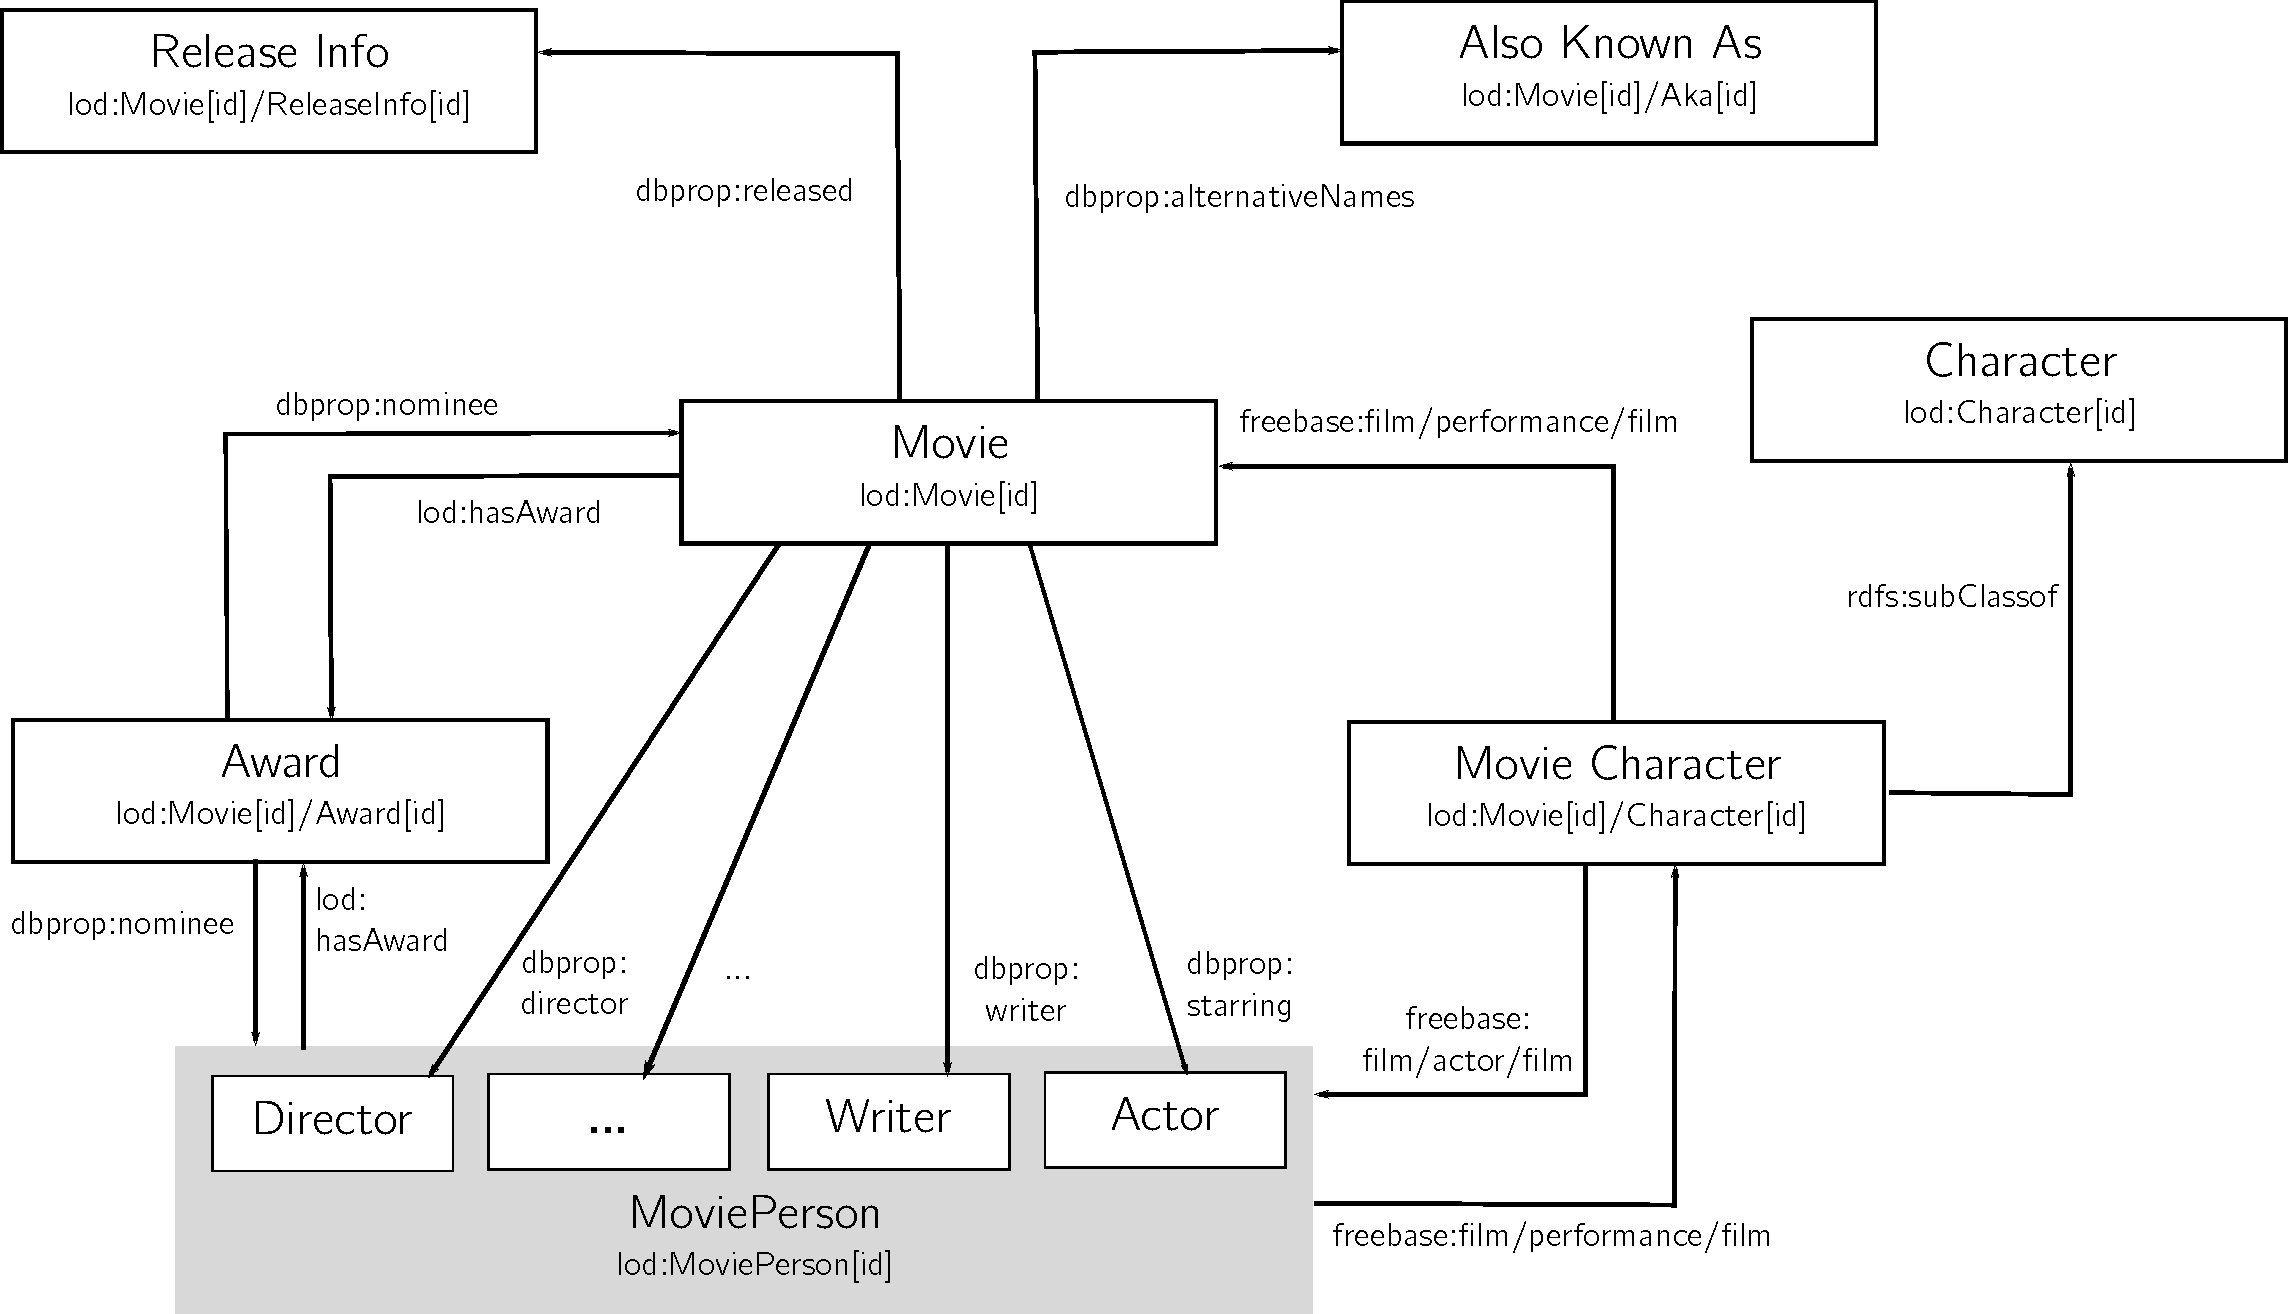
\includegraphics[width=\textwidth]{images/ontology.pdf}
\caption{Ontology}
\label{fig_ontology}
\end{figure}

The naive way to express roles, shown in Figure \ref{fig_ontology}, was one \emph{character} class which is connected to the corresponding movie (via film/performance) and actor (actor or performance).
This means that a role which exists in multiple movies (e.g. "cleaning lady") is one resource with an \emph{actor} property for each actor who has portrayed this role at some point. 

This approach caused problems in some cases.
For example an actor played a certain role in an old movie and also appears in the movies newer remake.
But now they play a different role while another act plays their original role. 
An example for this is the movie "Starsky and Hutch" (year), which is a remake of the (decade) TV series with the same name.
In the movie, both actors which originally portrayed Starsky and Hutch get a cameo appearance alongside the new cast for their old roles.
With the naive approach you do not know who played the Starsky role in the remake, because only references to the movies and the actors are given.

Therefore a additional class \emph{MovieCharacter} was introduced.
The resources of this class knows exactly one movie and all actors playing this role in this one movie.
The \emph{MovieCharacter} has a connection, named \emph{Character}, to the \emph{Character} class, which describes the general role.
This means that the \emph{MovieCharacter} in the "Starsky and Hutch" example is "starksyStarskyAndHutch1970" and the \emph{Character} is "starksy".

%onthology -> movie character (james bond- john connory), classes, picture presentation, dbpedia-props > freebase > own